\section{Results}
\label{sec:results}

We organise the results into three subsections matching the
experimental design (\secref{sec:harnesses}): E1 (fine-tuning, sweep
over $N$), E2 (\rag, sweep over $N$ with model-family axis), and E3
(diversity-axis comparison at fixed $N{=}4$). \mvp estimates and
slope-significance tests are reported per metric.

\subsection{E1: Fine-tuning ecosystem}
\label{sec:results_e1}

\para{Headline.}
Even at $N{=}16$, the perplexity of \distilgpt copies retraining on
their own pooled outputs continues to climb monotonically over six
iterations. The \emph{rate} of climb falls $\sim 5\times$ from $N{=}1$
to $N{=}16$, but no $N$ tested has a slope statistically
indistinguishable from zero. \mvp on perplexity at $T{=}6$ is
$\mathbf{N{=}4}$ under the half-collapse criterion of
\secref{sec:problem}; on the higher-better metrics no $N$ qualifies.

\para{Perplexity dynamics.}
\tabref{tab:e1_perp} reports perplexity at each iteration for each $N$.
The $N{=}1$ baseline replicates \citet{shumailov2024nature}: perplexity
goes from $66.4$ to $495.2$ over six iterations, a $\mathbf{7.45\times}$
collapse. The diversity benefit per $N$-doubling is non-monotonic: most
of the gain is concentrated at $N{=}1{\to}N{=}2$ (collapse multiplier
drops from $7.45\times$ to $4.43\times$, $-40\%$) and at
$N{=}8{\to}N{=}16$ (from $3.03\times$ to $2.10\times$, $-31\%$);
intermediate doublings each contribute only $\sim 17{-}18\%$.

\begin{table}[t]
    \centering
    \caption{E1 perplexity (mean across agents) on \wikitext test, by
    population size $N$ and iteration $t$. Mean $\pm$ std across two
    seeds. Best (lowest) terminal perplexity in \textbf{bold}.}
    \label{tab:e1_perp}
    \resizebox{\textwidth}{!}{%
    \begin{tabular}{@{}rccccccc@{}}
        \toprule
        $N$ & $t{=}0$ & $t{=}1$ & $t{=}2$ & $t{=}3$ & $t{=}4$ & $t{=}5$ & $t{=}6$ \\
        \midrule
        1   & 66.4 \tiny{$\pm$0.0} & 87.6 \tiny{$\pm$2.1} & 125.5 \tiny{$\pm$5.3} & 180.6 \tiny{$\pm$2.9} & 248.3 \tiny{$\pm$7.9} & 362.2 \tiny{$\pm$35.7} & 495.2 \tiny{$\pm$57.8} \\
        2   & 69.6 \tiny{$\pm$0.2} & 87.9 \tiny{$\pm$0.4} & 117.3 \tiny{$\pm$0.5} & 153.7 \tiny{$\pm$0.9} & 196.8 \tiny{$\pm$3.7} & 253.6 \tiny{$\pm$2.4}  & 308.4 \tiny{$\pm$2.4}  \\
        4   & 75.0 \tiny{$\pm$0.0} & 91.1 \tiny{$\pm$0.3} & 118.8 \tiny{$\pm$1.8} & 152.6 \tiny{$\pm$3.5} & 188.4 \tiny{$\pm$3.6} & 232.0 \tiny{$\pm$2.9}  & 275.1 \tiny{$\pm$12.0} \\
        8   & 81.0 \tiny{$\pm$0.1} & 95.7 \tiny{$\pm$0.3} & 119.5 \tiny{$\pm$0.5} & 148.3 \tiny{$\pm$0.6} & 180.4 \tiny{$\pm$2.1} & 210.4 \tiny{$\pm$0.7}  & 245.4 \tiny{$\pm$4.3}  \\
        16  & 85.8 \tiny{$\pm$0.1} & 93.9 \tiny{$\pm$0.2} & 108.8 \tiny{$\pm$0.1} & 126.0 \tiny{$\pm$0.8} & 143.7 \tiny{$\pm$1.2} & 161.9 \tiny{$\pm$0.9}  & \textbf{180.5} \tiny{$\pm$0.6} \\
        \bottomrule
    \end{tabular}
    }
\end{table}

\para{Slope tests.}
\tabref{tab:e1_slopes} reports the OLS slope of perplexity on iteration.
Every $N$ has a slope significantly greater than zero ($p < 10^{-3}$).
The slope falls from $69.9$ ppl/iter at $N{=}1$ to $16.3$ ppl/iter at
$N{=}16$, a $4.3\times$ reduction. \figref{fig:e1_perp} visualises the
trajectories; \figref{fig:e1_mvp} plots the relationship between $N$
and terminal perplexity, the curve that defines \mvp on this metric.

\begin{table}[t]
    \centering
    \caption{E1 perplexity slope (per iteration) by population size,
    estimated by OLS over $T{=}6$ iterations. All slopes are
    statistically significant at $p < 10^{-3}$.}
    \label{tab:e1_slopes}
    \begin{tabular}{@{}rcc@{}}
        \toprule
        $N$ & slope (ppl/iter) & $p$-value \\
        \midrule
        1   & 69.9 \tiny{$\pm$17.6} & $5.6 \times 10^{-4}$ \\
        2   & 40.3 \tiny{$\pm$ 6.1} & $4.8 \times 10^{-5}$ \\
        4   & 34.0 \tiny{$\pm$ 4.0} & $1.5 \times 10^{-5}$ \\
        8   & 28.0 \tiny{$\pm$ 2.7} & $5.0 \times 10^{-6}$ \\
        16  & \textbf{16.3} \tiny{$\pm$ 1.4} & $\mathbf{3.1 \times 10^{-6}}$ \\
        \bottomrule
    \end{tabular}
\end{table}

\begin{figure}[t]
    \centering
    \begin{subfigure}[b]{0.48\textwidth}
        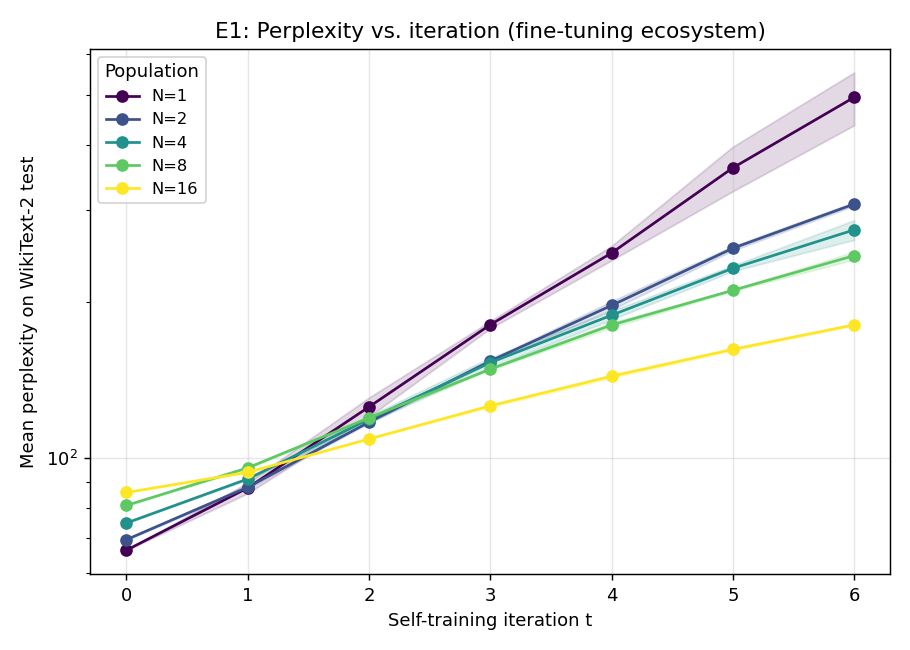
\includegraphics[width=\linewidth]{figures/finetune_perplexity_vs_iter.png}
        \caption{Perplexity trajectories.}
        \label{fig:e1_perp}
    \end{subfigure}
    \hfill
    \begin{subfigure}[b]{0.48\textwidth}
        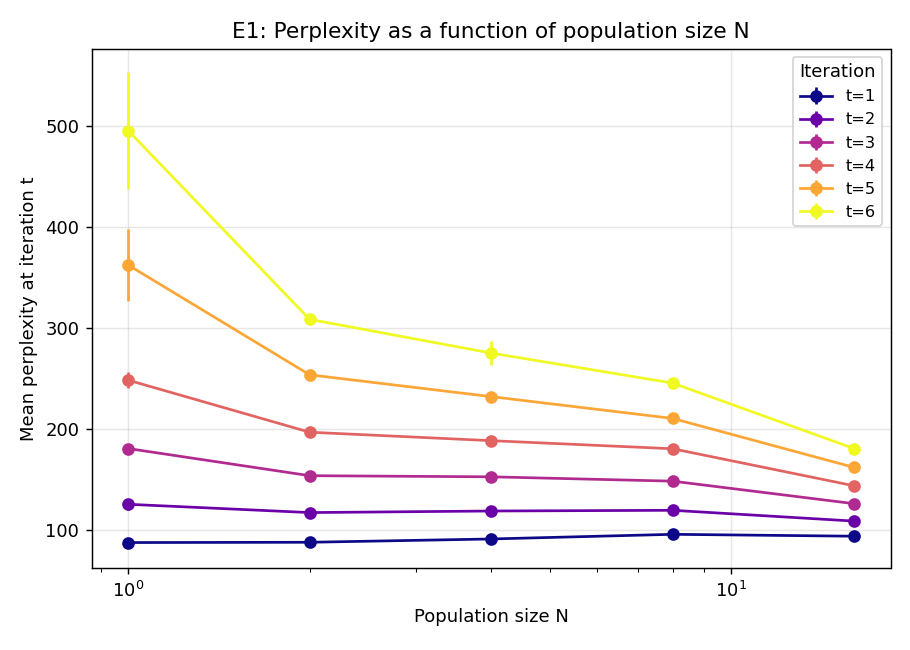
\includegraphics[width=\linewidth]{figures/finetune_mvp_curve.png}
        \caption{Terminal perplexity vs $N$.}
        \label{fig:e1_mvp}
    \end{subfigure}
    \caption{E1 fine-tuning ecosystem. \figleft Perplexity rises
    monotonically at every $N$; the $N{=}1$ curve reproduces the
    canonical Shumailov collapse signature. \figright The
    $N$--vs--terminal-perplexity curve does not flatten: more agents
    always help, but no finite $N \le 16$ halts collapse over $T{=}6$
    iterations.}
    \label{fig:e1_overview}
\end{figure}

\para{Lexical and semantic diversity.}
\figref{fig:e1_div} shows distinct-bigram, mean pairwise distance, and
\hsd over the same runs. The same $N$ ordering applies: more agents
preserve more diversity, but no $N$ flattens. Distinct-bigram and
mean-pairwise-distance slopes are negative and significant for every
$N$; consequently no $N$ qualifies as the \mvp on these
higher-better metrics under the slope criterion.

\begin{figure}[t]
    \centering
    \begin{subfigure}[b]{0.32\textwidth}
        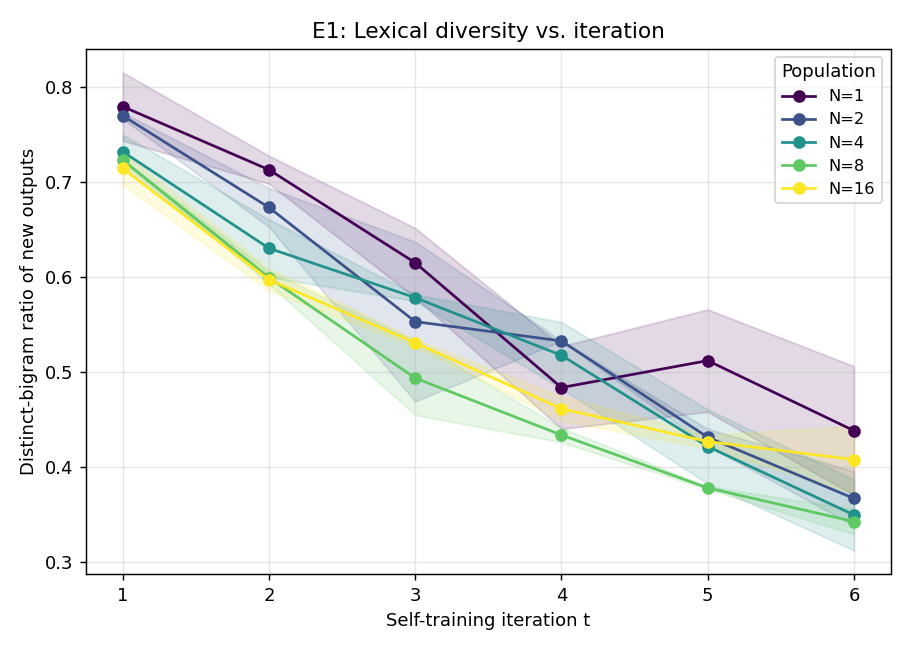
\includegraphics[width=\linewidth]{figures/finetune_distinct2_vs_iter.png}
        \caption{Distinct-2.}
        \label{fig:e1_d2}
    \end{subfigure}
    \begin{subfigure}[b]{0.32\textwidth}
        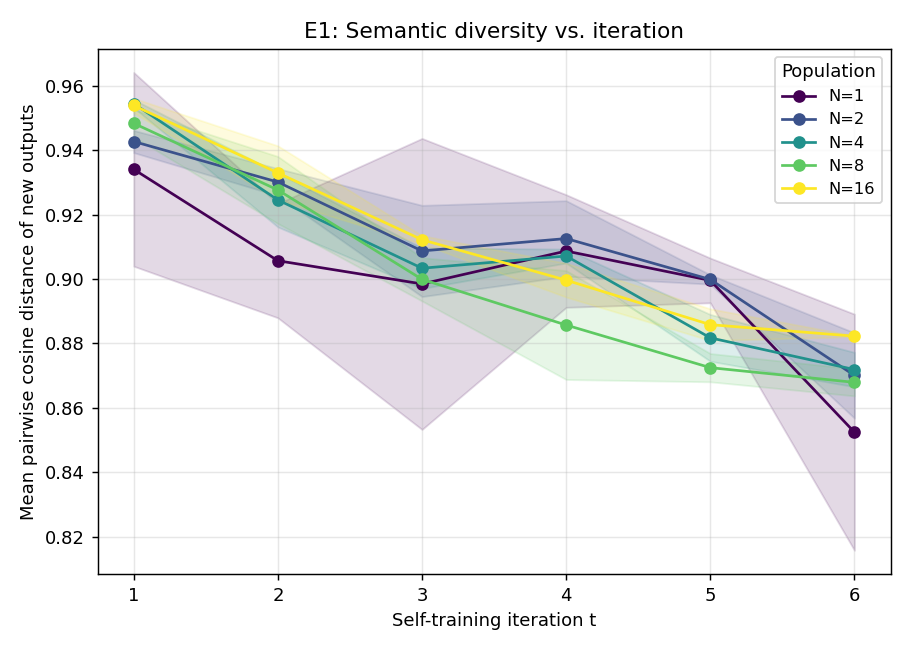
\includegraphics[width=\linewidth]{figures/finetune_meanpd_vs_iter.png}
        \caption{Mean pairwise distance.}
        \label{fig:e1_mpd}
    \end{subfigure}
    \begin{subfigure}[b]{0.32\textwidth}
        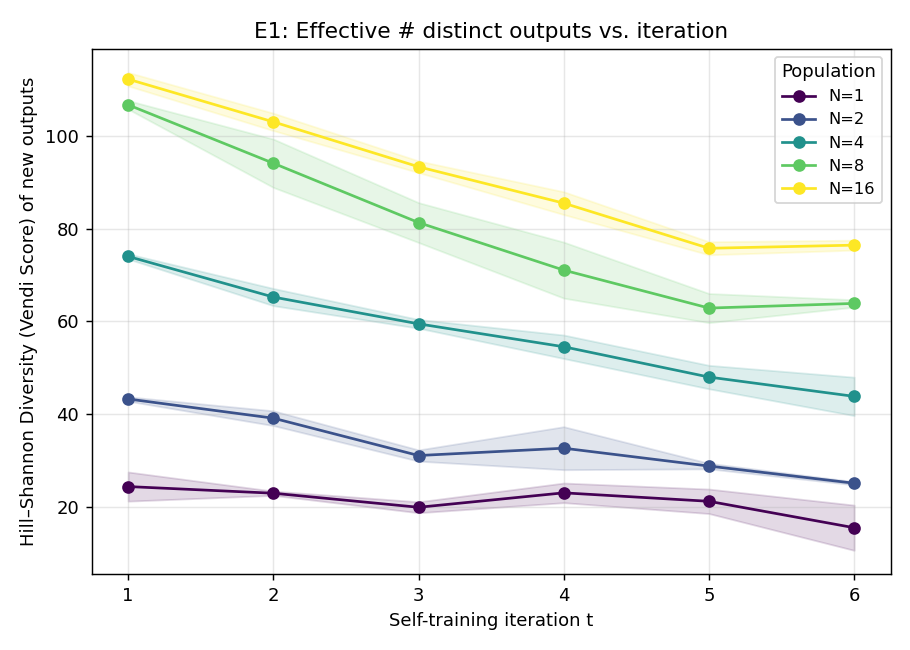
\includegraphics[width=\linewidth]{figures/finetune_hsd_vs_iter.png}
        \caption{Hill--Shannon Diversity.}
        \label{fig:e1_hsd}
    \end{subfigure}
    \caption{E1 diversity metrics. Larger $N$ delays decay on all three
    diversity dimensions, but every $N$ tested still shows a
    statistically significant downward slope.}
    \label{fig:e1_div}
\end{figure}

\subsection{E2: \rag ecosystem (model-family axis)}
\label{sec:results_e2}

\para{Headline.}
Two LLMs from different pretraining families, sharing a growing
retrieval pool, preserve full diversity over $T{=}12$ iterations:
both \hsd and mean pairwise distance have regression slopes
indistinguishable from zero ($p \approx 0.4$). \mvp on mean pairwise
distance at $T{=}12$ is $\mathbf{N{=}2}$.

\para{Diversity by $N$.}
\tabref{tab:e2_main} reports diversity at iteration 1 and at the
terminal iteration. At $N{=}2$ the mean pairwise distance is
essentially constant ($0.89 \to 0.90$); at $N{=}3$ it drifts down by
$0.07$ over twelve iterations; at $N{=}4$ it loses only $0.04$. The
per-iteration regression slopes (\tabref{tab:e2_slopes}) are negative
but not statistically significant for any $N$.

\begin{table}[t]
    \centering
    \caption{E2 diversity at iteration 1 and at terminal iteration $T$
    in the \rag harness with model-family differentiation.
    Mean $\pm$ std across three seeds. $N{=}1{,}2{,}3$ ran to $T{=}12$;
    $N{=}4$ to $T{=}10$. \hsd@$t{=}1$ for $N{=}1$ is $1.00$ by
    construction (single agent; inter-agent metrics are $0$).}
    \label{tab:e2_main}
    \resizebox{\textwidth}{!}{%
    \begin{tabular}{@{}rrcccccc@{}}
        \toprule
        $N$ & $T$ & \hsd@1 & meanPD@1 & Frob@1 & \hsd@$T$ & meanPD@$T$ & Frob@$T$ \\
        \midrule
        1 & 12 & 1.00 & 0.00 & 0.00 & 1.00 & 0.00 & 0.00 \\
        2 & 12 & 1.99 \tiny{$\pm$0.01} & 0.89 \tiny{$\pm$0.04} & 1.25 \tiny{$\pm$0.06} & 1.99 \tiny{$\pm$0.00} & \textbf{0.90} \tiny{$\pm$0.01} & 1.27 \tiny{$\pm$0.01} \\
        3 & 12 & 2.81 \tiny{$\pm$0.14} & 0.81 \tiny{$\pm$0.08} & 2.01 \tiny{$\pm$0.16} & 2.63 \tiny{$\pm$0.24} & 0.74 \tiny{$\pm$0.09} & 1.91 \tiny{$\pm$0.17} \\
        4 & 10 & 3.32 \tiny{$\pm$0.27} & 0.79 \tiny{$\pm$0.04} & 2.87 \tiny{$\pm$0.08} & 3.15 \tiny{$\pm$0.20} & 0.75 \tiny{$\pm$0.02} & \textbf{2.77} \tiny{$\pm$0.02} \\
        \bottomrule
    \end{tabular}
    }
\end{table}

\begin{table}[t]
    \centering
    \caption{E2 OLS slopes of diversity metrics on iteration in the
    \rag harness with model-family axis. None of these slopes is
    significantly different from zero at $p < 0.05$.}
    \label{tab:e2_slopes}
    \begin{tabular}{@{}rlcc@{}}
        \toprule
        $N$ & metric & slope (per iter) & $p$-value \\
        \midrule
        2 & \hsd                & $-0.0004 \pm 0.0008$ & 0.407 \\
        2 & mean pairwise dist. & $-0.0016 \pm 0.0038$ & 0.439 \\
        3 & \hsd                & $-0.0101 \pm 0.0150$ & 0.215 \\
        3 & mean pairwise dist. & $-0.0043 \pm 0.0047$ & 0.107 \\
        4 & \hsd                & $-0.0170 \pm 0.0194$ & 0.125 \\
        4 & mean pairwise dist. & $-0.0042 \pm 0.0041$ & 0.082 \\
        \bottomrule
    \end{tabular}
\end{table}

\begin{figure}[t]
    \centering
    \begin{subfigure}[b]{0.32\textwidth}
        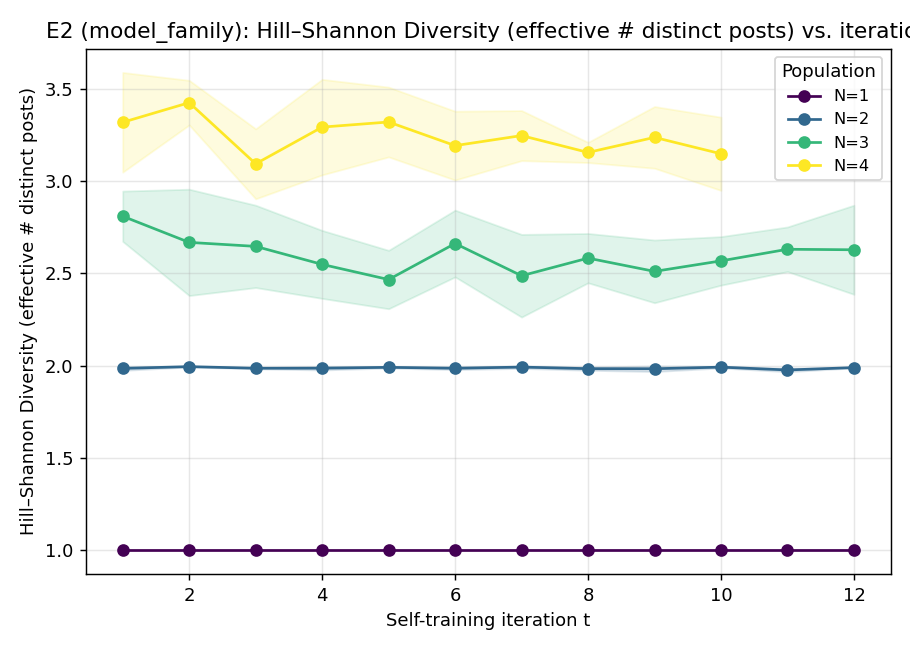
\includegraphics[width=\linewidth]{figures/rag_model_family_hsd_vs_iter.png}
        \caption{\hsd.}
        \label{fig:e2_hsd}
    \end{subfigure}
    \begin{subfigure}[b]{0.32\textwidth}
        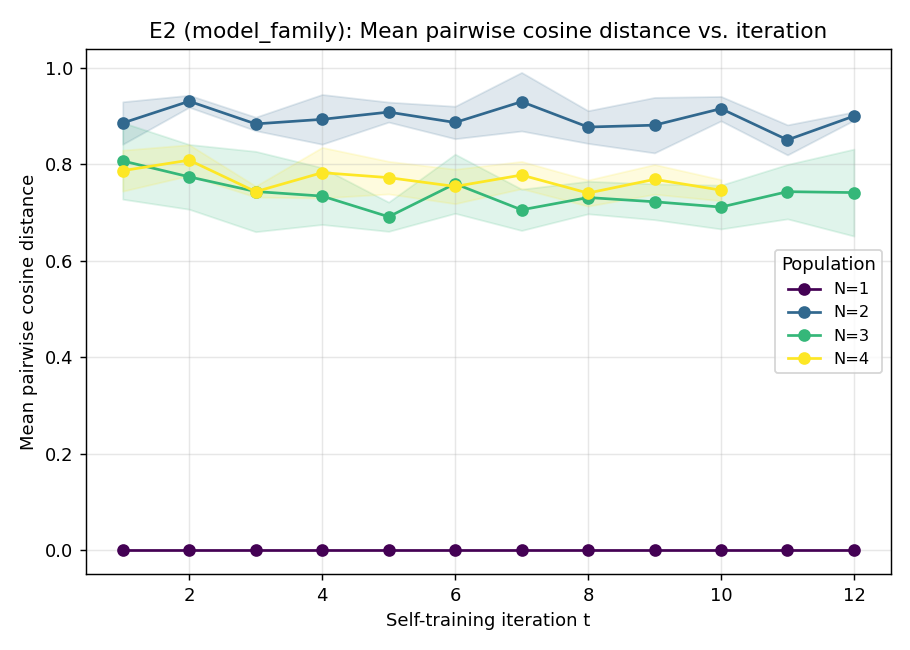
\includegraphics[width=\linewidth]{figures/rag_model_family_meanpd_vs_iter.png}
        \caption{Mean pairwise dist.}
        \label{fig:e2_mpd}
    \end{subfigure}
    \begin{subfigure}[b]{0.32\textwidth}
        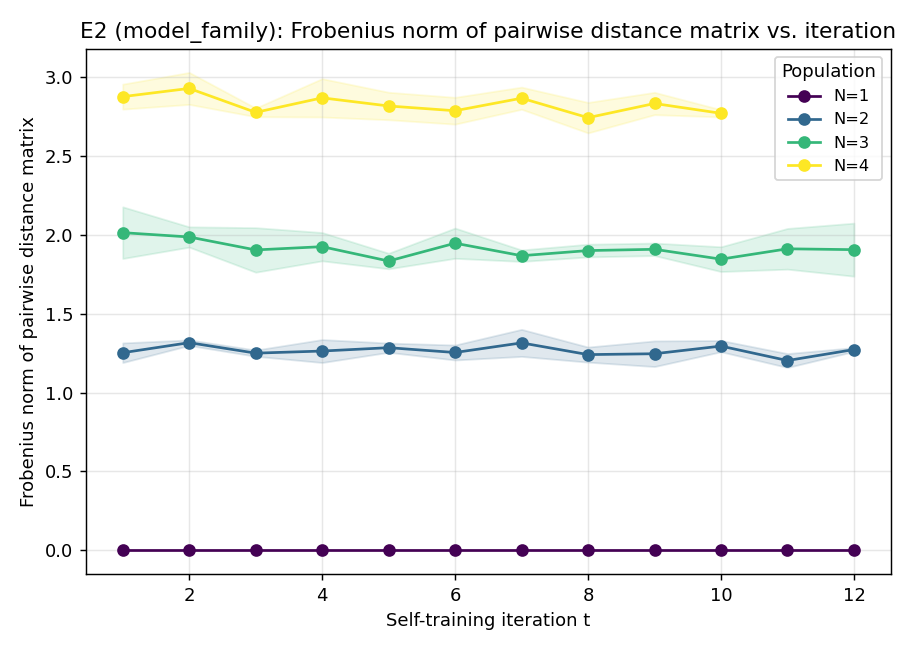
\includegraphics[width=\linewidth]{figures/rag_model_family_frob_vs_iter.png}
        \caption{Frobenius norm.}
        \label{fig:e2_frob}
    \end{subfigure}
    \caption{E2 \rag-ecosystem trajectories under model-family
    differentiation. Diversity is essentially flat at $N{=}2$ and only
    weakly decaying at $N{=}3$ and $N{=}4$; contrast with the
    monotone collapse of E1 (\figref{fig:e1_overview}).}
    \label{fig:e2_overview}
\end{figure}

\subsection{E3: Diversity-axis comparison at $N{=}4$}
\label{sec:results_e3}

\para{Headline.}
Holding $N{=}4$ fixed, model-family differentiation preserves
\textbf{1.9$\times$} the terminal inter-agent semantic distance of the
next-best axis. The other three axes (\axisseed, \axisdata,
\axisprompt) are essentially indistinguishable.

\para{Axis ranking.}
\tabref{tab:e3_main} reports diversity at $t{=}1$ and $t{=}10$ for
each axis. The terminal mean-pairwise-distance ranking is
\axisfamily $(0.75) \gg$ \axisdata $(0.40) \approx$ \axisprompt $(0.40)
> $ \axisseed $(0.32)$.
\figref{fig:e3_terminal} plots the terminal values directly: the
model-family bar towers above the others by roughly a factor of two.

\begin{table}[t]
    \centering
    \caption{E3 diversity-axis comparison at fixed $N{=}4$. Mean $\pm$
    std across three seeds; $T{=}10$. \axisfamily preserves
    \textbf{1.9$\times$} the terminal mean pairwise distance of the
    next-best axis.}
    \label{tab:e3_main}
    \resizebox{\textwidth}{!}{%
    \begin{tabular}{@{}lcccccc@{}}
        \toprule
        axis           & \hsd@1 & meanPD@1 & Frob@1 & \hsd@10 & meanPD@10 & Frob@10 \\
        \midrule
        \axisseed       & 3.03 \tiny{$\pm$0.32} & 0.56 \tiny{$\pm$0.11} & 1.98 \tiny{$\pm$0.41} & 2.23 \tiny{$\pm$0.28} & 0.32 \tiny{$\pm$0.07} & 1.14 \tiny{$\pm$0.26} \\
        \axisdata       & 2.63 \tiny{$\pm$0.50} & 0.46 \tiny{$\pm$0.15} & 1.67 \tiny{$\pm$0.55} & 2.45 \tiny{$\pm$0.20} & 0.40 \tiny{$\pm$0.08} & 1.48 \tiny{$\pm$0.35} \\
        \axisprompt     & 2.68 \tiny{$\pm$0.34} & 0.49 \tiny{$\pm$0.16} & 1.78 \tiny{$\pm$0.66} & 2.45 \tiny{$\pm$0.45} & 0.40 \tiny{$\pm$0.13} & 1.42 \tiny{$\pm$0.47} \\
        \axisfamily     & \textbf{3.32} \tiny{$\pm$0.27} & \textbf{0.79} \tiny{$\pm$0.04} & \textbf{2.87} \tiny{$\pm$0.08} & \textbf{3.15} \tiny{$\pm$0.20} & \textbf{0.75} \tiny{$\pm$0.02} & \textbf{2.77} \tiny{$\pm$0.02} \\
        \bottomrule
    \end{tabular}
    }
\end{table}

\begin{figure}[t]
    \centering
    \begin{subfigure}[b]{0.32\textwidth}
        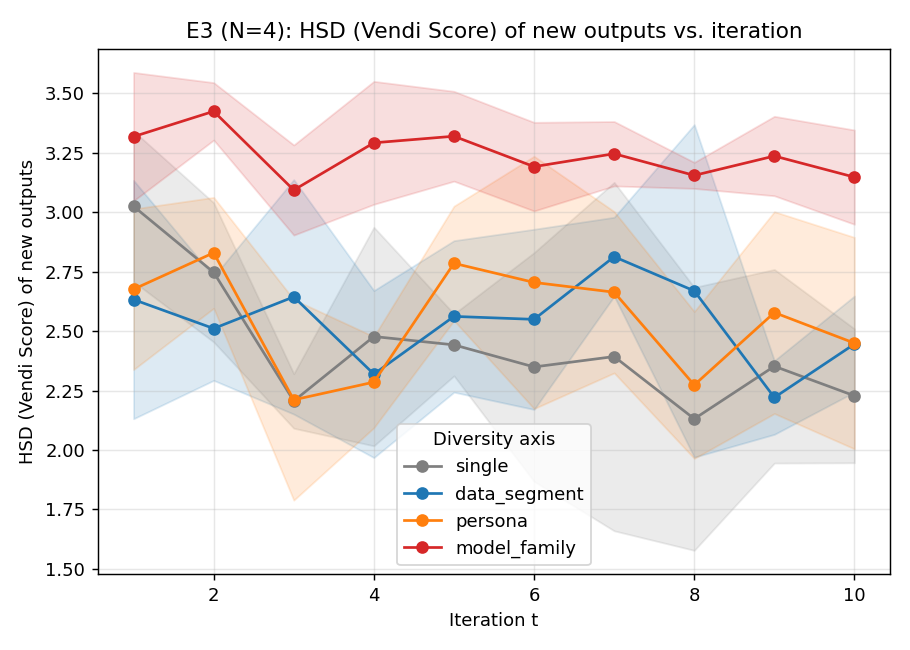
\includegraphics[width=\linewidth]{figures/axis_compare_hsd.png}
        \caption{\hsd over time.}
        \label{fig:e3_hsd}
    \end{subfigure}
    \begin{subfigure}[b]{0.32\textwidth}
        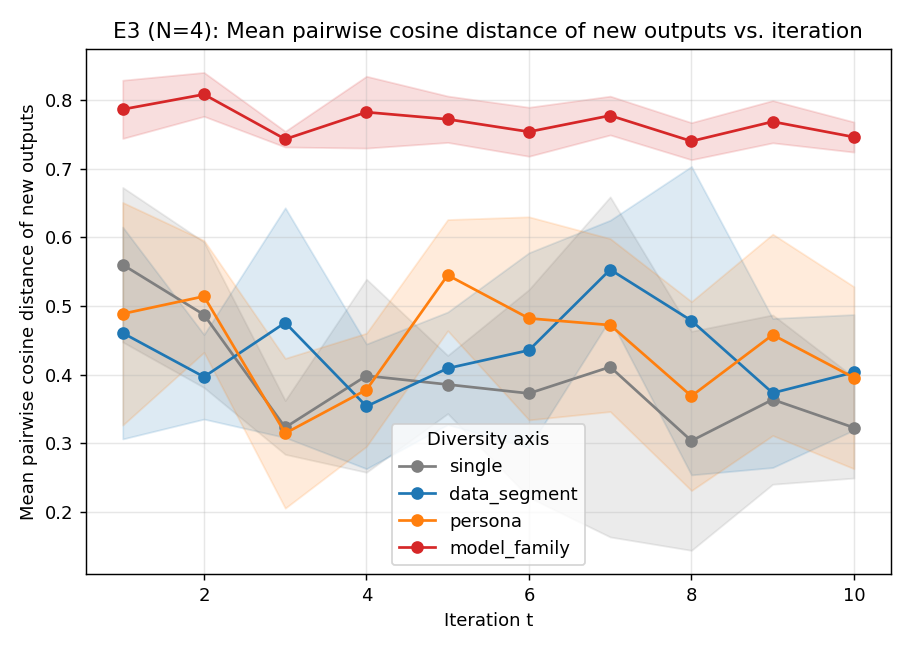
\includegraphics[width=\linewidth]{figures/axis_compare_meanpd.png}
        \caption{Mean pairwise dist.\ over time.}
        \label{fig:e3_mpd}
    \end{subfigure}
    \begin{subfigure}[b]{0.32\textwidth}
        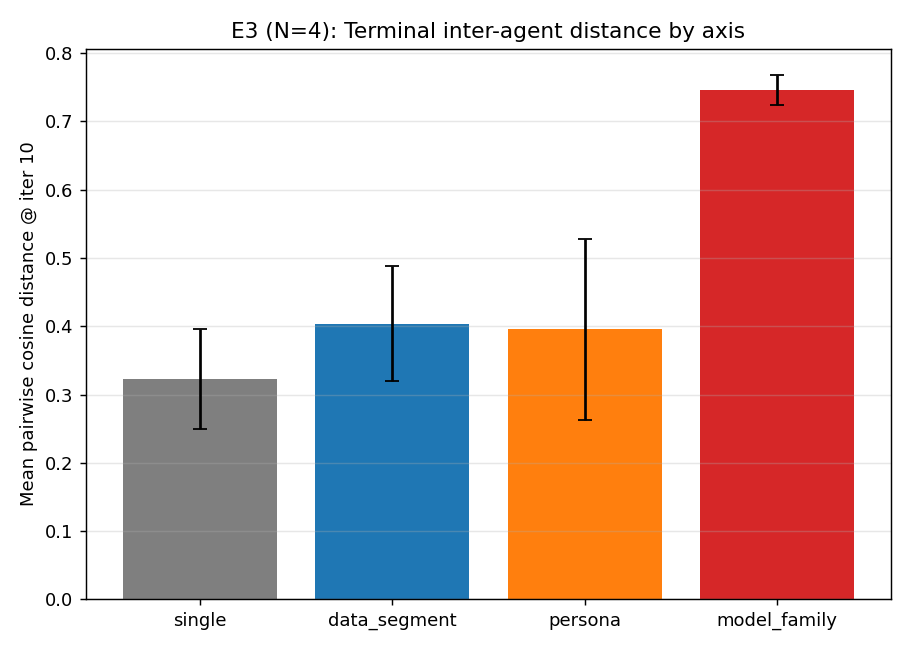
\includegraphics[width=\linewidth]{figures/axis_compare_terminal_meanpd.png}
        \caption{Terminal mean PD by axis.}
        \label{fig:e3_terminal}
    \end{subfigure}
    \caption{E3 axis comparison at $N{=}4$. \axisfamily (model-family
    diversity) is the only axis whose terminal inter-agent semantic
    distance separates from the rest; \axisprompt and \axisdata are
    essentially indistinguishable from the same-everything-different-
    seeds control \axisseed.}
    \label{fig:e3_overview}
\end{figure}

\subsection{Cross-experiment summary}

\tabref{tab:mvp} consolidates \mvp estimates across both harnesses and
the metrics for which they are well-defined. The two harnesses give
different answers: in the parameter-frozen \rag operationalisation
$\mvp = 2$ on the model-family axis; in the parameter-updating
fine-tuning operationalisation, no $N \le 16$ halts collapse on the
slope criterion, though $N{=}4$ is enough to limit terminal perplexity
to half the $N{=}1$ catastrophe.

\begin{table}[t]
    \centering
    \caption{\mvp estimates across experiments. ``None'' indicates no
    tested $N$ qualifies. ``Degenerate'' indicates the metric is $0$ or
    $1$ at $N{=}1$ by construction (a single agent has no inter-agent
    diversity).}
    \label{tab:mvp}
    \begin{tabular}{@{}llcc@{}}
        \toprule
        experiment & metric & \mvp & direction \\
        \midrule
        E1 & perplexity                              & 4         & lower better \\
        E1 & distinct-2                              & none      & higher better \\
        E1 & mean pairwise dist.                     & none      & higher better \\
        E2 ($\axisfamily$) & mean pairwise dist.\ at $T{=}12$ & \textbf{2} & higher better \\
        E2 ($\axisfamily$) & \hsd at $T{=}12$        & degenerate at $N{=}1$ & higher better \\
        \bottomrule
    \end{tabular}
\end{table}
